\chapter{Metodología de la Investigación}
\section{Diseño de la investigación}
El diseño de esta investigación es de tipo cuasi-experimental, ya que se observará la relación entre las marcas en los bordes de la lengua (variable independiente) y la presencia de bruxismo (variable dependiente) en niños, sin manipular el entorno ni asignar condiciones al azar. Las imágenes de las lenguas serán procesadas mediante técnicas de visión computacional para extraer características clave, que luego serán evaluadas mediante modelos de deep learning. Este enfoque permite analizar patrones asociados al bruxismo de forma controlada y sistemática, sin alterar las condiciones naturales de los participantes.

\subsection{Alcance de la investigación}
El nivel de esta investigación es explicativo, ya que se busca desarrollar una aplicación móvil que permita el prediagnóstico de bruxismo en niños mediante el análisis de imágenes de sus lenguas. El sistema de visión computacional que se propone está diseñado para identificar patrones específicos, como las marcas en los bordes de la lengua, los cuales podrían estar asociados a esta condición. Este enfoque permite establecer una relación de causa-efecto, donde la presencia de ciertos patrones en las imágenes analizadas puede servir como indicador preliminar de bruxismo, facilitando una detección temprana y preventiva.

\subsection{Enfoque de la investigación}
El enfoque de esta investigación es cuantitativo, ya que se busca obtener datos medibles para el prediagnóstico de bruxismo en niños. Para esto, se emplearán imágenes de lenguas de niños con posibles signos de bruxismo, específicamente marcas en los bordes, que serán procesadas mediante técnicas de visión computacional. Los resultados obtenidos serán datos numéricos que permitirán entrenar modelos de deep learning para identificar patrones asociados al bruxismo. Estos modelos se utilizarán como herramienta de apoyo para el prediagnóstico, aportando precisión y rapidez en la detección de esta condición en una etapa temprana.

\subsection{Población}
La población de esta investigación está constituida por individuos que presentan posibles señales de bruxismo, específicamente aquellos con marcas en los bordes de la lengua identificadas mediante examen visual o imágenes clínicas.

\subsection{Muestra}
La muestra utilizada en esta investigación consiste en un conjunto de 1250 imágenes de lenguas marcadas y no marcadas, obtenidas de la plataforma kaggle, de las cuales todas fueron tomadas de personas con posibles señales de bruxismo.

\section{Operacionalización de variables}
En este apartado se describen las principales variables del estudio, detallando su definición conceptual, definición operacional, los indicadores asociados, así como el instrumento y la escala utilizada para su medición. Estas variables permiten estructurar y guiar el proceso de análisis basado en técnicas de aprendizaje profundo.

\begin{table}[H]
\centering
\caption{Definición de variables del estudio.}
\label{tabla:variables}
\begin{tabular}{|p{2.5cm}|p{3cm}|p{3.5cm}|p{2.5cm}|p{2.5cm}|p{1.5cm}|}
\hline
\textbf{Variable} & \textbf{Definición Conceptual} & \textbf{Definición Operacional} & \textbf{Indicadores} & \textbf{Instrumento} & \textbf{Escala} \\ \hline
\textbf{Marcas en los bordes de la lengua} & Signos visuales en el borde de la lengua indicativos de bruxismo. & Detección de marcas en imágenes procesadas mediante técnicas de visión computacional. & Presencia o ausencia de marcas. & Modelo de \textit{deep learning}. & Nominal \\ \hline
\textbf{Presencia de bruxismo} & Apretamiento o rechinamiento involuntario de dientes, identificado por signos en lengua. & Diagnóstico preliminar basado en patrones visuales asociados al bruxismo. & Predicción del modelo. & Modelo de \textit{deep learning}. & Nominal \\ \hline
\end{tabular}
\end{table}

\section{Técnicas de recolección de datos}
En esta sección se describen las técnicas utilizadas para la obtención y el procesamiento de los datos necesarios para el desarrollo del modelo de aprendizaje profundo. Se detalla la fuente de datos, el proceso de recolección y las herramientas empleadas en el análisis.

\begin{table}[H]
    \caption{Técnicas de recolección de datos.}
    \centering
    \renewcommand{\arraystretch}{1.5} % Aumenta el espacio entre filas
    \setlength{\tabcolsep}{8pt} % Ajusta el espacio entre columnas
    \begin{tabular}{|p{4cm}|p{10cm}|}
        \hline
        \textbf{Técnica} & \textbf{Descripción} \\ \hline
        Fuente de datos & 1250 imágenes de lenguas marcadas y no marcadas obtenidas de Kaggle. \\ \hline
        Proceso de recolección & Selección, preprocesamiento y etiquetado de las imágenes para la detección de marcas indicativas de bruxismo. \\ \hline
        Herramientas utilizadas & Visión computacional para detección de características y \textit{deep learning} para análisis y clasificación de imágenes. \\ \hline
    \end{tabular}
\end{table}


\section{Metodología de Implementación de la Solución}

La metodología propuesta para implementar un modelo de \textit{Deep Learning} está basada en el ciclo de vida de desarrollo de modelos de Inteligencia Artificial, con adaptaciones específicas para abordar el diagnóstico de bruxismo en niños mediante patrones de sonido y frecuencia, así como el análisis de imágenes de lengua.

Para este caso, se busca desarrollar un modelo de \textit{Deep Learning} que asista en el prediagnóstico de bruxismo infantil. La metodología propuesta toma como referencia algunos enfoques presentados en los antecedentes revisados, adaptándolos para el análisis de datos de sonido y procesamiento de imágenes relacionadas con marcas en los bordes de la lengua. En la Figura \ref{3:fig301} se presenta de manera gráfica la metodología propuesta para este proyecto.

\begin{figure}[H]
	\begin{center}
		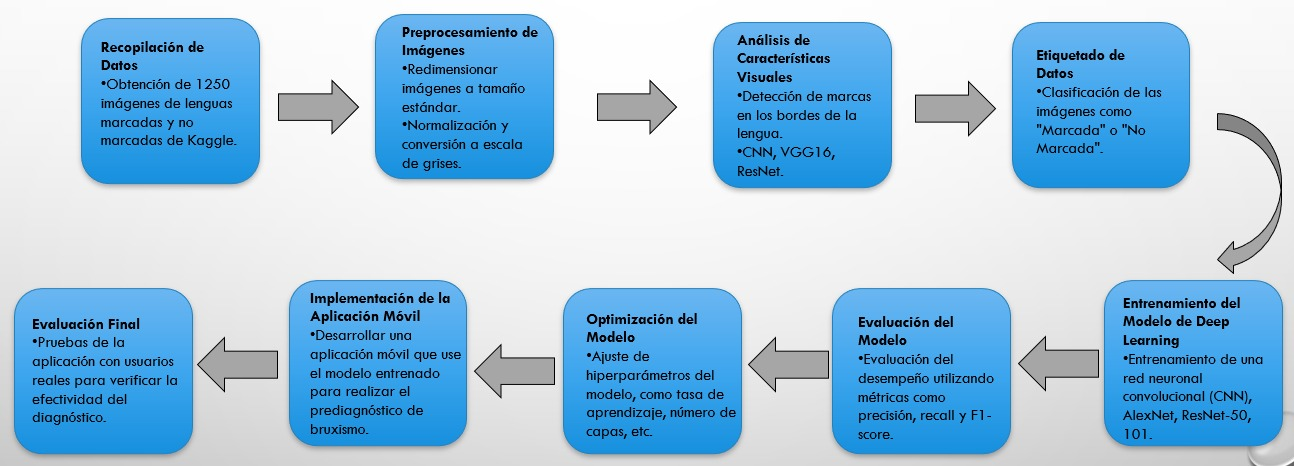
\includegraphics[width=1.00\textwidth]{3/figures/1.jpeg}
		\caption[Metodología de implementación]{Metodología de implementación. \\
		Fuente: Elaboración propia.}
		\label{3:fig301}
	\end{center}
\end{figure}




